\documentclass[border=6pt]{standalone}
\usepackage{tikz}
\usetikzlibrary{arrows.meta,positioning,shapes.geometric}
\begin{document}
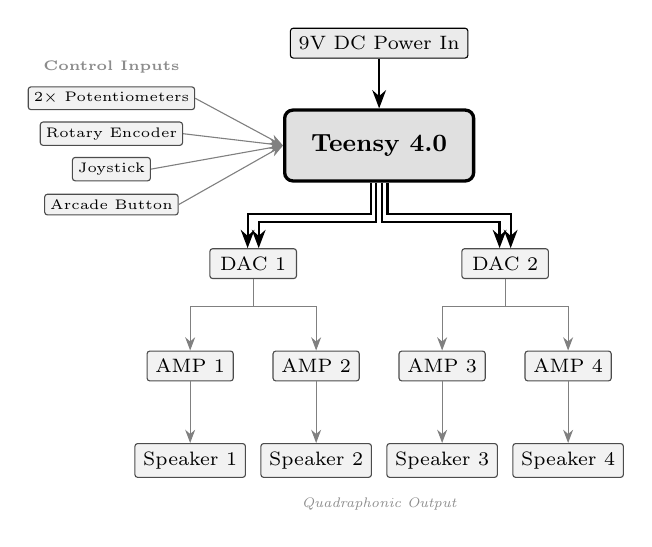
\begin{tikzpicture}

\node[rectangle, draw, fill=black!8, rounded corners=1pt, font=\scriptsize, inner sep=3pt] (pwr) at (0, 0) {9V DC Power In};

\node[rectangle, draw, very thick, fill=black!12, rounded corners=3pt, font=\small\bfseries, inner sep=4pt, minimum height=0.9cm, minimum width=2.4cm] (teensy) at (0, -1.3) {Teensy 4.0};

\draw[-Stealth, thick] (pwr) -- (teensy);

\node[rectangle, draw=black!70, fill=black!5, rounded corners=1pt, font=\tiny, inner sep=2pt] (c1) at (-3.4, -0.7) {2$\times$ Potentiometers};
\node[rectangle, draw=black!70, fill=black!5, rounded corners=1pt, font=\tiny, inner sep=2pt] (c2) at (-3.4, -1.15) {Rotary Encoder};
\node[rectangle, draw=black!70, fill=black!5, rounded corners=1pt, font=\tiny, inner sep=2pt] (c3) at (-3.4, -1.6) {Joystick};
\node[rectangle, draw=black!70, fill=black!5, rounded corners=1pt, font=\tiny, inner sep=2pt] (c4) at (-3.4, -2.05) {Arcade Button};

\draw[-Stealth, thin, black!50] (c1.east) -- (teensy.west);
\draw[-Stealth, thin, black!50] (c2.east) -- (teensy.west);
\draw[-Stealth, thin, black!50] (c3.east) -- (teensy.west);
\draw[-Stealth, thin, black!50] (c4.east) -- (teensy.west);

\node[font=\tiny\bfseries, text=black!45] at (-3.4, -0.3) {Control Inputs};

\node[rectangle, draw=black!70, fill=black!5, rounded corners=1pt, font=\scriptsize, inner sep=3pt, minimum width=1.1cm] (dac1) at (-1.6, -2.8) {DAC 1};
\node[rectangle, draw=black!70, fill=black!5, rounded corners=1pt, font=\scriptsize, inner sep=3pt, minimum width=1.1cm] (dac2) at (1.6, -2.8) {DAC 2};

\draw[-Stealth, thick] ([xshift=-3pt]teensy.south) -- ++(0,-0.4) -| ([xshift=-2pt]dac1.north);
\draw[-Stealth, thick] ([xshift=-1pt]teensy.south) -- ++(0,-0.5) -| ([xshift=2pt]dac1.north);
\draw[-Stealth, thick] ([xshift=1pt]teensy.south) -- ++(0,-0.5) -| ([xshift=-2pt]dac2.north);
\draw[-Stealth, thick] ([xshift=3pt]teensy.south) -- ++(0,-0.4) -| ([xshift=2pt]dac2.north);

\node[rectangle, draw=black!70, fill=black!5, rounded corners=1pt, font=\scriptsize, inner sep=3pt, minimum width=0.9cm] (amp1) at (-2.4, -4.1) {AMP 1};
\node[rectangle, draw=black!70, fill=black!5, rounded corners=1pt, font=\scriptsize, inner sep=3pt, minimum width=0.9cm] (amp2) at (-0.8, -4.1) {AMP 2};
\node[rectangle, draw=black!70, fill=black!5, rounded corners=1pt, font=\scriptsize, inner sep=3pt, minimum width=0.9cm] (amp3) at (0.8, -4.1) {AMP 3};
\node[rectangle, draw=black!70, fill=black!5, rounded corners=1pt, font=\scriptsize, inner sep=3pt, minimum width=0.9cm] (amp4) at (2.4, -4.1) {AMP 4};

\draw[-Stealth, thin, black!50] (dac1.south) -- ++(0,-0.35) -| (amp1.north);
\draw[-Stealth, thin, black!50] (dac1.south) -- ++(0,-0.35) -| (amp2.north);
\draw[-Stealth, thin, black!50] (dac2.south) -- ++(0,-0.35) -| (amp3.north);
\draw[-Stealth, thin, black!50] (dac2.south) -- ++(0,-0.35) -| (amp4.north);

\node[rectangle, draw=black!70, fill=black!5, rounded corners=1pt, font=\scriptsize, inner sep=3pt, minimum width=1.1cm] (sp1) at (-2.4, -5.3) {Speaker 1};
\node[rectangle, draw=black!70, fill=black!5, rounded corners=1pt, font=\scriptsize, inner sep=3pt, minimum width=1.1cm] (sp2) at (-0.8, -5.3) {Speaker 2};
\node[rectangle, draw=black!70, fill=black!5, rounded corners=1pt, font=\scriptsize, inner sep=3pt, minimum width=1.1cm] (sp3) at (0.8, -5.3) {Speaker 3};
\node[rectangle, draw=black!70, fill=black!5, rounded corners=1pt, font=\scriptsize, inner sep=3pt, minimum width=1.1cm] (sp4) at (2.4, -5.3) {Speaker 4};

\draw[-Stealth, thin, black!50] (amp1) -- (sp1);
\draw[-Stealth, thin, black!50] (amp2) -- (sp2);
\draw[-Stealth, thin, black!50] (amp3) -- (sp3);
\draw[-Stealth, thin, black!50] (amp4) -- (sp4);

\node[font=\tiny\itshape, text=black!45] at (0, -5.85) {Quadraphonic Output};

\end{tikzpicture}
\end{document}
